%%%%%%%%%%%%%%%%%%%%%%%%%%%%%%%%%%%%%%%%%
% Beamer Presentation
% LaTeX Template
% Version 1.0 (10/11/12)
%
% This template has been downloaded from:
% http://www.LaTeXTemplates.com
%
% License:
% CC BY-NC-SA 3.0 (http://creativecommons.org/licenses/by-nc-sa/3.0/)
%
%%%%%%%%%%%%%%%%%%%%%%%%%%%%%%%%%%%%%%%%%

%----------------------------------------------------------------------------------------
%	PACKAGES AND THEMES
%----------------------------------------------------------------------------------------

\documentclass{beamer}

\mode<presentation> {

% The Beamer class comes with a number of default slide themes
% which change the colors and layouts of slides. Below this is a list
% of all the themes, uncomment each in turn to see what they look like.

%\usetheme{default}
%\usetheme{AnnArbor}
%\usetheme{Antibes}
%\usetheme{Bergen}
%\usetheme{Berkeley}
%\usetheme{Berlin}
%\usetheme{Boadilla}
%\usetheme{CambridgeUS}
%\usetheme{Copenhagen}
%\usetheme{Darmstadt}
%\usetheme{Dresden}
%\usetheme{Frankfurt}
%\usetheme{Goettingen}
%\usetheme{Hannover}
%\usetheme{Ilmenau}
%\usetheme{JuanLesPins}
%\usetheme{Luebeck}
\usetheme{Madrid}
%\usetheme{Malmoe}
%\usetheme{Marburg}
%\usetheme{Montpellier}
%\usetheme{PaloAlto}
%\usetheme{Pittsburgh}
%\usetheme{Rochester}
%\usetheme{Singapore}
%\usetheme{Szeged}
%\usetheme{Warsaw}

% As well as themes, the Beamer class has a number of color themes
% for any slide theme. Uncomment each of these in turn to see how it
% changes the colors of your current slide theme.

%\usecolortheme{albatross}
%\usecolortheme{beaver}
%\usecolortheme{beetle}
%\usecolortheme{crane}
%\usecolortheme{dolphin}
%\usecolortheme{dove}
%\usecolortheme{fly}
%\usecolortheme{lily}
%\usecolortheme{orchid}
%\usecolortheme{rose}
%\usecolortheme{seagull}
%\usecolortheme{seahorse}
%\usecolortheme{whale}
%\usecolortheme{wolverine}

%\setbeamertemplate{footline} % To remove the footer line in all slides uncomment this line
%\setbeamertemplate{footline}[page number] % To replace the footer line in all slides with a simple slide count uncomment this line

%\setbeamertemplate{navigation symbols}{} % To remove the navigation symbols from the bottom of all slides uncomment this line
}
\newcommand{\R}{\mathbb{R}}
\usepackage{graphicx} % Allows including images
\usepackage{booktabs} % Allows the use of \toprule, \midrule and \bottomrule in tables
\usepackage[brazilian]{babel}
\usepackage[utf8]{inputenc}
\usepackage[T1]{fontenc}
\usepackage{listings}
\usepackage{hyperref}
\hypersetup{
    colorlinks=true,
    linkcolor=blue,
    filecolor=magenta,      
    urlcolor=cyan,
}

\usepackage{listings}
\usetheme{metropolis}
\urlstyle{same}
\graphicspath{ {figuras/} }
%----------------------------------------------------------------------------------------
%	TITLE PAGE
%----------------------------------------------------------------------------------------

\title{Modelos Sequencias para Regressão em Séries Temporais} % The short title appears at the bottom of every slide, the full title is only on the title page

\author{Thiago Lira} % Your name
\institute[IME-USP] % Your institution as it will appear on the bottom of every slide, may be shorthand to save space
{
Instituto de Matemática e Estatística - USP \\ % Your institution for the title page
\medskip
\textit{thlira15@gmail.com} % Your email address
}
\date{\today} % Date, can be changed to a custom date

\begin{document}

\begin{frame}
\titlepage % Print the title page as the first slide
\end{frame}

\begin{frame}
\frametitle{Overview} % Table of contents slide, comment this block out to remove it
\tableofcontents % Throughout your presentation, if you choose to use \section{} and \subsection{} commands, these will automatically be printed on this slide as an overview of your presentation
\end{frame}



\begin{frame}
%%% A durabilidade e vida útil do cimento tem sido o problema mais importante enfrentado
%%% pela indústria de construção civil nas últimas décadas (Taffese e Sistonen, 2017). Os
%%% custos de manutenção são da ordem de bilhões de dólares e portanto, a capacidade da
%%% previsão de propriedades do cimento desde a sua produção ganha grande importância.
%%% Une-se a isso a presença cada vez maior de métodos de ML em domínios diversos da
%%% engenharia e ciência e surge então a tentativa de usar algoritmos de aprendizado também
%%% para esse domínio (Baykasoğlu et al., 2004, Öztaş et al., 2006).
%%% slide cimento histrico 
\end{frame}



\begin{frame}
%%% slide cimento foto do processo com numeros DECORA FDP
\end{frame}


\section{Análise dos Dados}

\begin{frame}
%%% plot com numero de entradas faltando nos dados 
\begin{figure}[H]
\centering
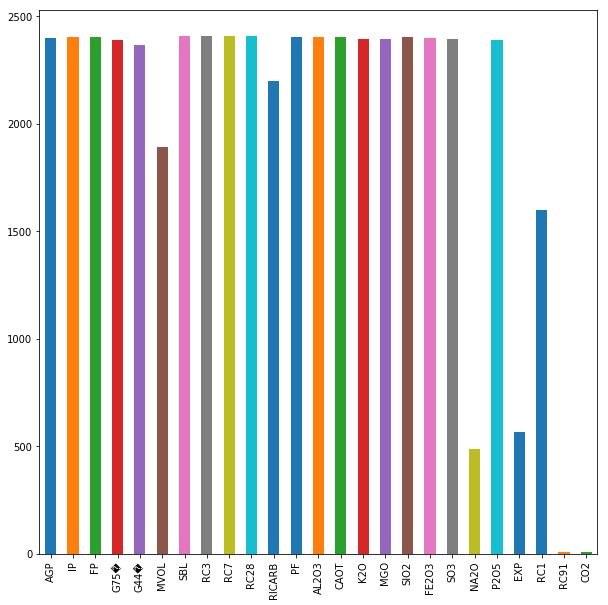
\includegraphics[scale=0.3]{slides_dados_faltando}
\caption{Dados faltantes em cada coluna dos dados de Expedição de Cimento}
\end{figure}

\end{frame}

\begin{frame}
%%% slide apenas do RC3,RC7 e RC28
\begin{figure}[H]
\centering
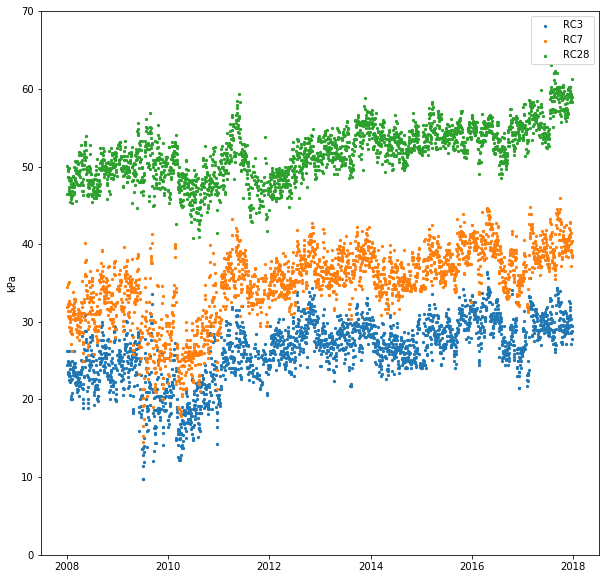
\includegraphics[scale=0.4]{slides_dados}
\caption{Dados que serão usados para o problema de Regressão}
\end{figure}

\end{frame}


\begin{frame}
%%% slide com tabela de correlação
\begin{table}[H]
\centering
\begin{tabular}{l|lll}
\cline{2-4}
\textbf{}                  & \multicolumn{1}{l|}{RC3} & \multicolumn{1}{l|}{RC7} & \multicolumn{1}{l|}{RC28} \\ \hline
\multicolumn{1}{|l|}{RC3}  & 1                        & 0.734201                 & 0.388973                  \\ \cline{1-1}
\multicolumn{1}{|l|}{RC7}  & 0.734201                 & 1                        & 0.484725                  \\ \cline{1-1}
\multicolumn{1}{|l|}{RC28} & 0.388973                 & 0.484725                 & 1                         \\ \cline{1-1}
\end{tabular}
\caption{Correlação entre Índices de Resistência dos dados de
  Expedição de Cimento}
\label{corr3728}
\end{table}

\end{frame}

\begin{frame}
%%% slide com analise FFT só do RC28
\end{frame}

\begin{frame}
%%% slide definindo aprendizado supervisionado/regressao
\end{frame}

\begin{frame}
%%% slide mostrando rede neural (mesmo diagrama da quali)
\end{frame}

\begin{frame}
%%% slide definindo série temporal/sequencial
\end{frame}

\begin{frame}
%%% slide definindo uma LSTM
\end{frame}

\begin{frame}
%%% slide com modelo Uber
\end{frame}

\begin{frame}
%%% slide inferencia bayesiana com a integral e os caralho
\end{frame}

\begin{frame}
%%% slide com dropout imagem da quali
\end{frame}

\begin{frame}
%%% slide do modelo da uber com zoom
\end{frame}

\begin{frame}
%%% formulas de variancia no modelo uber
\end{frame}

\begin{frame}
%%% resultados modelos não-sequenciais
\end{frame}

\begin{frame}
%%% resultados modelo uber
\end{frame}

\begin{frame}
%%% conclusão até agora
\end{frame}

\begin{frame}
%%% direção futura imagem do cronograma
\end{frame}















\end{document}